% -*- TeX-engine: xetex -*-

\documentclass[xetex,aspectratio=169,14pt,hyperref={pdfpagelabels=true,pdflang={en-GB}}]{beamer}

\usepackage[sci,noslidestrathidentity]{strathclyde}
\strathsetidentity{Department of}{Computer \& Information Sciences}

\usepackage{lmodern}
\usepackage{subscript}
\usepackage{url}
\usepackage{pifont}
\usepackage{csquotes}
\usepackage{mathpartir}
\usepackage{stmaryrd}
\usepackage{multirow}
\usepackage{euler}
\usepackage[normalem]{ulem}

% 2013-09-08 SU adding xetex specifics
% http://www.woggie.net/2008/07/16/beamer-pdftex-and-xetex/
\usepackage{xltxtra}

% 2013-09-08 SU http://robjhyndman.com/hyndsight/xelatex/
\defaultfontfeatures{Ligatures=TeX}

% 2015-12-09 SU table beautified
\renewcommand{\arraystretch}{1.2}
\usepackage{booktabs}

%MGK compatibility
\newcommand{\hh}[1]
  {\medskip\textbf{\large #1}}
\newcommand{\pdu}[3]
  {#1\rightarrow #2 : &\ & \makebox[70mm][l]{$#3$}}



\setlength{\marginparwidth}{2cm}
\usepackage{todonotes}%[disable]
\let\OldTodo\todo
\renewcommand{\todo}{\OldTodo[inline]}%
\newcommand{\todolater}[1]{}% Things to do for next year


\DeclareTextCommandDefault{\nobreakspace}{\leavevmode\nobreak\ }
\usepackage{rotating}

\usepackage{pdfcomment}% To add alt text for images using \pdftooltip{}

\usepackage{appendixnumberbeamer}

\newcommand{\messageframe}[1]{\begin{frame}\begin{center}\Huge #1\end{center}\end{frame}}
\newcommand{\sechead}[1]{{\bf #1} \\}
\newcommand{\examplehead}[1]{{\bf Example:} {\it\textcolor{red!90}{#1}} \\}
\newcommand{\eqnote}[1]{\hspace{3cm}\textit{#1}}
\newcommand{\sidenote}[1]{\qquad {\footnotesize \textcolor{black!60}{(#1)}}}
\newcommand{\sem}[1]{\llbracket #1 \rrbracket}
\newcommand{\true}{\mathsf{T}}
\newcommand{\false}{\mathsf{F}}

\def\strikeafter<#1>#2{\temporal<#1>{#2}{\sout{#2}}{\sout{#2}}}


%\newcommand{\rhighlight}{\textcolor{titlered}}
\newcommand{\rhighlight}{\textbf}
\newcommand{\highlight}{\textbf}

% \setmainfont{Linux Biolinum O}
\setmainfont{LinBiolinum}[
Path=,
UprightFont = *_R.otf ,
BoldFont = *_RB.otf ,
ItalicFont = *_RI.otf
]

\setbeamertemplate{navigation symbols}{}
%\usecolortheme[rgb={0.8,0,0}]{structure}
\usefonttheme{serif}
\usefonttheme{structurebold}
\setbeamercolor{description item}{fg=black}


\author[Atkey]{Dr.~Robert Atkey}
\institute[Strathclyde]{Computer \& Information Sciences}
\date[]{}

\newcommand{\weeksection}[1]{%
  \section{\thetitle{}, Part~\thesection : #1}
  \begin{frame}
    \begin{center}
      \textcolor{black!60}{\thetitle{}, Part \thesection}\\
      {\Huge #1}
    \end{center}
  \end{frame}}

\newcommand{\weektitle}[2]{\def\thetitle{#2}
\title[CS208 - Topic #1]{CS208 (Semester 1) Topic #1 : #2}}

\newcommand{\assigned}{:}

\newcommand{\forcedto}{\assigned_f}
\newcommand{\decideto}{\assigned_d}


\weektitle{5}{Specification and Verification}

\begin{document}

\frame{\titlepage}

\weeksection{Program Specification}

\begin{frame}
  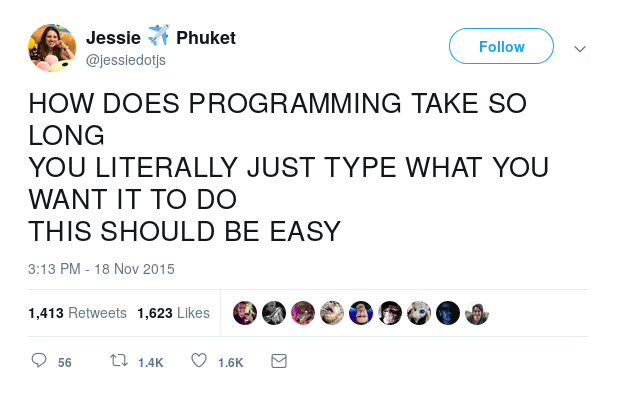
\includegraphics[width=0.8\textwidth]{tweet.png}

  {\small\url{https://twitter.com/jessiedotjs/status/667118579075141632}}
\end{frame}

\begin{frame}
  {From the birth of programming...}

  \begin{quotation}
    By June 1949 people had begun to realize that it was not so easy
    to get programs right as at one time appeared. I well remember
    when this realization first came on me with full force.

    ...
  \end{quotation}
\end{frame}

\begin{frame}
  {From the birth of programming...}

  \begin{quotation}
    ...

    The EDSAC was on the top floor of the building and the
    tape-punching and editing equipment one floor below. [...] It was
    on one of my journeys between the EDSAC room and the punching
    equipment that ``hesitating at the angles of stairs'' the
    realization came over me with full force that a \rhighlight{good
      part of the remainder of my life was going to be spent in
      finding errors in my own programs.}
  \end{quotation}
  Maurice Wilkes\\
  Memoirs of a Computer Pioneer, MIT Press, 1985, p. 145.

  \sidenote{The EDSAC was an early ``stored program''
    computers, and first ran in May 1949}
\end{frame}

\begin{frame}
  {What makes Programming Hard?}

  \begin{enumerate}
  \item Getting the syntax right? \\
    \sidenote{basically not a problem; loads of IDE support}

    \bigskip
  \item Needing Fancy Algorithms? \\
    \sidenote{Relatively rare to have to do something completely new}

    \bigskip
  \item Making sure it does the right thing? \\
    \sidenote{Validating the \emph{specification}}

    \bigskip
  \item Making sure you do it right? \\
    \sidenote{\emph{Verifying} the program against the Specification}
  \end{enumerate}
\end{frame}

\begin{frame}
  {Current best practice}

  \sidenote{An uncharitable caricature}

  \bigskip

  \begin{enumerate}
  \item Write or alter some code
  \item Test it
    % \sidenote{usually on a fixed set of test cases}\\
    % \sidenote{often written by the same person who wrote the code}
  \item Release it
  \item Users find bugs, or tell you that's not what they wanted
  \item Goto step 1
  \end{enumerate}

  \bigskip

  You can rearrange the \sout{deckchairs} steps and call it Agile, or
  TDD, or Waterfall, or eXtreme Programming, or whatever.
\end{frame}

\begin{frame}
  {Specification}

  Implicit in the previous is the existence of some
  \emph{specification}.

  \bigskip

  Crude idea: there is a specification that tells us everything about what a program must do

  Better idea: there are overlapping specifications of different levels of detail covering different aspects of the system:
  \begin{enumerate}
  \item High level requirements: produces the ``right'' reports
  \item ``Non-functional'': performance
  \item ``Non-functional'': easy to use
  \item ``Non-functional'': is ``fun''
  \item Low-level: doesn't crash, if a function says it returns an
    integer, then it actually does, if a method says it sorts arrays
    then it actually sorts arrays, ...
  \end{enumerate}
\end{frame}

\begin{frame}
  {Can we Verify programs?}

  Given a program \texttt{C} and a specification $P$, can we:
  \begin{enumerate}
  \item Verify that \texttt{C} satisfies $P$...
  \item \emph{rigorously}...
  \item with \emph{no room for doubt}...
  \item \emph{easily}, \emph{cost effectively}, \emph{maintainably}...
  \end{enumerate}
\end{frame}

\begin{frame}
  {No}

  \begin{enumerate}
  \item Writing specifications is hard -- what should the code do? \\
    \sidenote{probably the hardest bit}\\
%    \sidenote{I really hate this damn machine / I wish that they would sell it \\ \quad\quad\quad It never does quite what I want / But only what I tell it}
  \item We always have to make assumptions (contra point 3) \\
    \sidenote{assume things about the OS, the hardware, the universe etc.}
  \item Programs are very, very big and complex \\
    \sidenote{and the proofs are often very boring}
  \item Currently, proving programs is time consuming and difficult.
  \end{enumerate}
\end{frame}

\begin{frame}
  \sechead{Nevertheless...}

  We're going to try. \\
  \sidenote{and we might learn something on the way...}
\end{frame}



\begin{frame}
  {Specifying Programs}

  Ways of specifying what programs do:
  \begin{enumerate}
  \item As equations (as in Ask)
  \item As it is done in Syrup, by a reference implementation
  \item Pre- and post-conditions
  \item Traces
  \item ...
  \end{enumerate}
\end{frame}

\begin{frame}
  {Pre- and Post-conditions}


\end{frame}

\begin{frame}
  {An Execution Predicate}
\end{frame}

\weeksection{Program Verification}

\weeksection{}

\end{document}
